\section{Equality in Baek's upper bound}\label{sec:equality}

Let $K\in\Kc_{\pi/2}$ with $\cA(K)=\abs\Gs$. By \cref{cor:Ki}, $K\in\Ki$. Write $K_0=\KG$ for Gerver's cap, $K_1=K$,
$h_i=h_{K_i}$ and $\Delta=h_1-h_0$; since both are caps with rotation angle $\pi/2$, $\Delta(\pi/2)=0$. Let
$\xi_0=\xi_G$ and $\xi_1=\xi_K$ be the canonical triples (\cref{sec:Q}), and $K_{1/2}$, $B_{1/2}$, $D_{1/2}$ the components of
$\xi_{1/2}=\tfrac12\xi_0+\tfrac12\xi_1$.

\subsection{Equality in the concavity of \texorpdfstring{$\cQ$}{Q}}

\begin{lemma}[equality in \texorpdfstring{$\cS$}{S}]\label{lem:equality}
For each of the four terms $\cM_K(a,b;\mathbf z_K)$ of $\cS_K$,
\[
  \cM_{K_{1/2}}\bigl(a,b;\mathbf z_{K_{1/2}}\bigr)=\tfrac12\cM_{K_0}\bigl(a,b;\mathbf z_{K_0}\bigr)+\tfrac12\cM_{K_1}\bigl(a,b;\mathbf z_{K_1}\bigr).
\]
\end{lemma}

\begin{proof}
By \cref{fact:Q}\ref{fact:Q:triple}, \ref{fact:Q:max}, $\abs\Gs=\cA(K)\le\cQ(\xi_1)\le\abs\Gs$, and
$\cQ(\xi_0)=\abs\Gs$, so $\cQ(\xi_0)=\cQ(\xi_1)=\abs\Gs$. The set $\cT$ is closed under Minkowski combinations, so $\xi_{1/2}\in\cT$.
By \cref{fact:Q}\ref{fact:Q:decomp},
$\cQ=\Lambda-\cS-\cR-\cL$ with $\Lambda$ convex-linear and the three terms convex, so $\cQ(\xi_{1/2})\ge\frac12\cQ(\xi_0)+\frac12\cQ(\xi_1)=\abs\Gs$, while
$\cQ(\xi_{1/2})\le\abs\Gs$ by \cref{fact:Q}\ref{fact:Q:max}. So equality holds, and since $\Lambda$ is convex-linear this says
\[
  \bigl[\cS_{K_{1/2}}-\tfrac12\cS_{K_0}-\tfrac12\cS_{K_1}\bigr]+\bigl[\cR_{B_{1/2}}-\tfrac12\cR_{B_0}-\tfrac12\cR_{B_1}\bigr]
  +\bigl[\cL_{D_{1/2}}-\tfrac12\cL_{D_0}-\tfrac12\cL_{D_1}\bigr]=0 .
\]
Each bracket is $\le0$ by convexity, so each is $0$. The first is the sum of the corresponding brackets of
the four terms of $\cS$, which are all $\le0$; so each of them is $0$.
\end{proof}

\subsection{Equal tangent displacements}

By \cref{fact:Q}\ref{fact:Q:decomp}, for each term the displacement $\varrho_{K,\mathbf z_K}(t)$ is convex-linear in $K$. Write
$\varrho_i=\varrho_{K_i,\mathbf z_{K_i}}$, so that $\varrho_{1/2}=\frac12(\varrho_0+\varrho_1)$ and
\[
  \tfrac12\varrho_0^2+\tfrac12\varrho_1^2-\varrho_{1/2}^2=\tfrac14(\varrho_0-\varrho_1)^2 .
\]
So the equality of \cref{lem:equality} reads
\begin{equation}\label{eq:gap}
  \tfrac18\int_a^b\bigl(\varrho_0(t)-\varrho_1(t)\bigr)^2\dd t=0 ,
\end{equation}
and $\varrho_0=\varrho_1$ almost everywhere on $[a,b]$. The four intervals are $(0,\varphi)$, $(\varphi,\pi/2-\varphi)$,
$(\pi/2-\varphi,\pi/2)$ and $(\pi/2,\pi)$; none contains $\pi/2$. On each of them both $K_i$ satisfy
condition~(1) of the injectivity condition, so by \cref{fact:arms}\ref{fact:arms:regular} the vertices $v^+_{K_i}$ and $v^-_{K_i}$
agree there, and by \cref{fact:convex}\ref{fact:convex:vertices} (one-sided continuity) they are continuous there; so $h_i$ is differentiable with the continuous derivative $h_i'(t)=\ip{v^+_{K_i}(t)}{v_t}$,
and $\varrho_0,\varrho_1$ are continuous. Hence $\varrho_0=\varrho_1$ \emph{everywhere} on $(a,b)$. We read this off for the two kinds of curves.

\begin{lemma}[the tangent equations]\label{lem:tangent}
Let $(a,b)$ be one of the four intervals.
\begin{enumerate}[label=(\alph*)]
\item\label{lem:tangent:l} Suppose that $\mathbf z_K=\mathbf l_K^T$ with $b\le T<a+\pi$. Then there are $p,q\in\R$ with
$\Delta(t)=p\cos t+q\sin t$ for $t\in[a,b]$, and $\Delta(T)=p\cos T+q\sin T$.
\item\label{lem:tangent:y} Suppose that $\mathbf z_K=\yy_K$ (the second term, $(a,b)=(\varphi,\pi/2-\varphi)$). Then
$\Delta(t)=\Delta(b)-\int_t^b\Delta(u+\pi/2)\dd u$ for $t\in[a,b]$.
\end{enumerate}
\end{lemma}

\begin{proof}
\ref{lem:tangent:l} For $t\in(a,b)$ we have $0<T-t<\pi$, and $\ip{\mathbf l_K^T(t)}{v_t}=(h_K(T)-h_K(t)\cos(T-t))/\sin(T-t)$, so
$\varrho_i(t)=\dfrac{h_i(T)-h_i(t)\cos(T-t)}{\sin(T-t)}-h_i'(t)$. The equality $\varrho_0=\varrho_1$ is
\[
  \sin(T-t)\Delta'(t)+\cos(T-t)\Delta(t)=\Delta(T).
\]
Then $\chi(t)=\bigl(\Delta(t)-\Delta(T)\cos(T-t)\bigr)/\sin(T-t)$ has $\chi'=\bigl[\Delta'\sin(T-t)+\Delta\cos(T-t)-\Delta(T)\bigr]/\sin^2(T-t)=0$ on $(a,b)$, so
$\chi\equiv\kappa$ and $\Delta(t)=\Delta(T)\cos(T-t)+\kappa\sin(T-t)=p\cos t+q\sin t$, with $p=\Delta(T)\cos T+\kappa\sin T$ and
$q=\Delta(T)\sin T-\kappa\cos T$; then $p\cos T+q\sin T=\Delta(T)$. By continuity this holds on $[a,b]$.

\ref{lem:tangent:y} Here $\ip{\yy_K(t)-v^+_K(t)}{v_t}=h_K(t+\pi/2)-h_K'(t)$, so $\varrho_0=\varrho_1$ says $\Delta'(t)=\Delta(t+\pi/2)$ on $(a,b)$. Integrate; $\Delta$ is continuous.
\end{proof}

\subsection{The cap is a horizontal translate}

\begin{proposition}[the difference of support functions]\label{prop:kernel}
$\Delta(t)=s\cos t$ for $t\in[0,\pi]$, where $s=-\Delta(\pi)$.
\end{proposition}

\begin{proof}
We solve the four equations in reverse order, using $\Delta(\pi/2)=0$.

On $[\pi/2,\pi]$ (target $T=\pi$): $\Delta=p\cos t+q\sin t$ and $\Delta(\pi/2)=q=0$, so $\Delta(t)=p\cos t$ and $\Delta(\pi)=-p$; thus
$\Delta(t)=s\cos t$ on $[\pi/2,\pi]$ with $s=-\Delta(\pi)$.

On $[\pi/2-\varphi,\pi/2]$ (target $T=\pi-\varphi$): $\Delta=p'\cos t+q'\sin t$, $\Delta(\pi/2)=q'=0$, and $\Delta(\pi-\varphi)=p'\cos(\pi-\varphi)$.
By the previous step $\Delta(\pi-\varphi)=s\cos(\pi-\varphi)$, and $\cos(\pi-\varphi)\ne0$, so $p'=s$.

On $[\varphi,\pi/2-\varphi]$: with $b=\pi/2-\varphi$, $\Delta(u+\pi/2)=s\cos(u+\pi/2)=-s\sin u$ for $u\in[\varphi,b]$ by the first
step, and $\Delta(b)=s\cos b$ by the second, so
$\Delta(t)=s\cos b+s\int_t^b\sin u\dd u=s\cos t$.

On $[0,\varphi]$ (target $T=\pi/2$): $\Delta=p''\cos t+q''\sin t$, $\Delta(\pi/2)=q''=0$, and $\Delta(\varphi)=s\cos\varphi=p''\cos\varphi$ gives $p''=s$.
\end{proof}

\begin{figure}[ht]
\centering
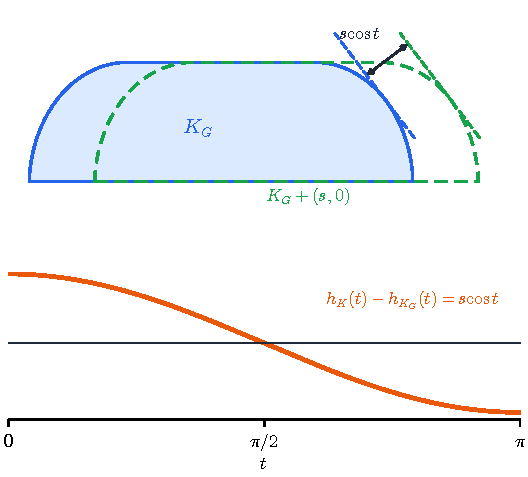
\includegraphics[width=0.74\linewidth]{figures/fig-translate}
\caption{\cref{prop:kernel,lem:translate}. Top: Gerver's cap $K_G$ and its horizontal translate by $(s,0)$; their supporting lines at the normal $t$
lie $s\cos t$ apart. Bottom: the difference $h_K-h_{K_G}=s\cos t$ of the support functions on $[0,\pi]$.}
\label{fig:translate}
\end{figure}

\begin{lemma}[caps with translated supports]\label{lem:translate}
If $K,C\in\Kc_{\pi/2}$ and $h_K(t)-h_C(t)=s\cos t$ for $t\in[0,\pi]$, then $K=C+(s,0)$ and
$K\setminus\cN(K)=(C\setminus\cN(C))+(s,0)$.
\end{lemma}

\begin{proof}
By \eqref{eq:cap-fan} with $\omega=\pi/2$, $K=\{p:\,p_y\ge0,\ \ip p{u_t}\le h_K(t)\text{ for }t\in[0,\pi]\}$, and likewise for $C$.
Since $h_{C+(s,0)}(t)=h_C(t)+s\cos t$ and $(s,0)$ is parallel to the floor, $C+(s,0)$ is the same set as $K$.
Finally $Q^-_{C+w}(t)=Q^-_C(t)+w$ and $F_{\pi/2}+(s,0)=F_{\pi/2}$.
\end{proof}

\begin{theorem}[maximizing right-angle caps]\label{thm:caps}
A cap $K\in\Kc_{\pi/2}$ has $\cA(K)=\abs\Gs$ if and only if $K=\KG+(s,0)$ for some $s\in\R$. In this case
$K\setminus\cN(K)=\Gs+(s,0)$. Consequently the maximizers of $\cA$ on $\Kc_{\pi/2}$ are the horizontal translates of Gerver's cap, and
every monotone sofa $U$ with rotation angle $\pi/2$ and $\abs U=\abs\Gs$ is a horizontal translate of $\Gs$.
\end{theorem}

\begin{proof}
If $\cA(K)=\abs\Gs$, then $K\in\Ki$ by \cref{cor:Ki}; \cref{prop:kernel} and \cref{lem:translate} (with $C=\KG$)
give $K=\KG+(s,0)$ and $K\setminus\cN(K)=(\KG\setminus\cN(\KG))+(s,0)=\Gs+(s,0)$ by \cref{fact:gerver}\ref{fact:gerver:cap}.
Conversely $\cA(\KG)=\abs\Gs$ by \cref{fact:monotone}\ref{fact:monotone:area}, and $\cA(C+(s,0))=\cA(C)$ for every cap $C$, since
$\cN(C+(s,0))=\cN(C)+(s,0)$. The maximum of $\cA$ is $\abs\Gs$ by \cref{fact:optimal}. If $U$ is a monotone
sofa with rotation angle $\pi/2$ and $\abs U=\abs\Gs$, its cap $K=\cC(U)$ has $\cA(K)=\abs U=\abs\Gs$
(\cref{fact:monotone}\ref{fact:monotone:area}), and $U=K\setminus\cN(K)$.
\end{proof}
